\documentclass{standalone}
\usepackage{tikz}
\usepackage{ctex,siunitx,bm}
\setCJKmainfont{Noto Serif CJK SC}
\usepackage{tkz-euclide,ninecolors}
\usepackage{amsmath}
\usetikzlibrary{patterns, calc}
\usetikzlibrary {decorations.pathmorphing, decorations.pathreplacing, decorations.shapes,}
\begin{document}
\small
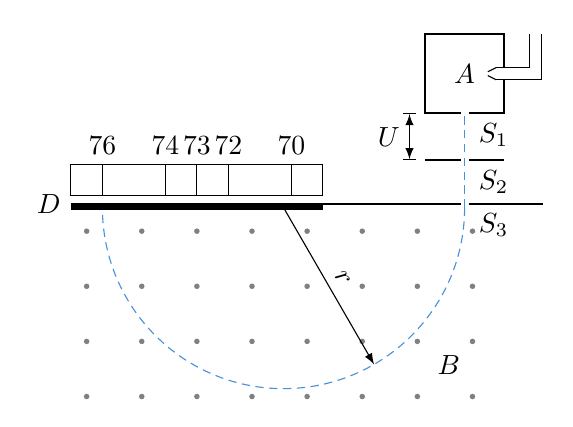
\begin{tikzpicture}[>=latex,yscale=1.0]
  \foreach \x in {0.1,-0.6,...,-5}
  {
    \foreach \y in {-0.3,-1.0,-1.7,-2.4}
    {
      \fill[gray](\x,\y)circle(1pt);
    }
  }
  \draw[densely dashed,azure6](0,0)--(0,1.2);
  % \draw[densely dashed,azure6](0,0)arc(0:-180:1.5);
  % \draw[densely dashed,azure6](0,0)arc(0:-180:1.7);
  \draw[densely dashed,azure6](0,0)arc(0:-180:2.3);
  \draw[->,thin](-2.3,0)--++(-60:2.3)node[midway,above,sloped]{$r$};
  \draw[thick](-0.05,0.05)--(-5,0.05)node[left]{$D$}(0.05,0.05)--(1,0.05)node[at start,below right]{$S_3$}(0.05,0.6)--(0.5,0.6)node[at start,below right]{$S_2$}(-0.05,0.6)--(-0.5,0.6)(0.05,1.2)--(0.5,1.2)node[at start,below right]{$S_1$}--(0.5,2.2)--(-0.5,2.2)--(-0.5,1.2)--(-0.05,1.2);
  \draw[double,double distance=4pt](0.4,1.7)--++(0.5,0)--++(0,0.5);
  \draw[thin]([yshift=2.2pt]0.4,1.7)--++(-3pt,-1.5pt)([yshift=-2.2pt]0.4,1.7)--++(-3pt,1.5pt);
  \node at (0,1.7){$A$};
  \foreach \x/\y in {-1.8/{},-2.2/70,-3/72,-3.4/73,-3.8/74,-4.6/76,-5.0/{}}
  {
    \draw[thin](\x,0.15)--(\x,0.55)node[above]{\y};
  }
  \draw[thin](-5,0.55)--(-1.8,0.55)(-5,0.15)--(-1.8,0.15);
  \draw[ultra thick](-5,0)--(-1.8,0);
  \draw[thin,|<->|](-0.7,0.6)--(-0.7,1.2)node[midway,left]{$U$};
  \node at (-0.2,-2.0){$B$};
\end{tikzpicture}
\end{document}